\icode{O-MD-CA-L2-261115-010}
如图所示，两个质量分别为 \(m_1\)和\(m_2\) 的物体 \(A\)、\(B\) 叠放在光滑水平面上，\(A\) 与 \(B\) 间的动摩擦因数为 \(\mu\)。当水平力恒力 \(F\) 作用于\(B\)，使\(A\)、\(B\)一起向右加速运动，求\(A\)、\(B\)之间摩擦力大小。

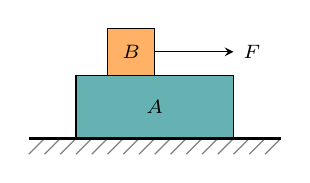
\begin{tikzpicture}[font=\scriptsize]
	\draw[fill=teal!60] (0,0) rectangle(2,.8)node[midway]{\(A\)};
	\draw[fill=orange!60] (.4,.8) rectangle(1,1.4)node[midway]{\(B\)};
	\draw[-stealth] (1,1.1)--++(1,0)node[right]{\(F\)};
	\foreach \x in {-.6,-.4,...,2.6}
		\draw[gray] (\x,-.2)--++(.2,.2);
	\draw[thick] (-.6,0)--(2.6,0);
\end{tikzpicture}
\begin{answer}
    
\end{answer}